\section{Networking}

\begin{figure}[htb]
  \centering
  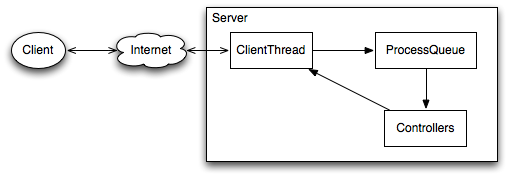
\includegraphics[width=0.8\textwidth]{network.png}
  \caption{Overview of Network Flow in Calico}
  \label{fig:network}
\end{figure}
% Intro parts
As a distributed and collaborative system, networking is a key part of Calico. The networking system must be able to support many clients at the same time, many of who may be working on the same workspace. The networking system in Calico consists of three major components: The main server socket and individual client process threads, the network queue processor, and the \texttt{CalicoPacket}. These three components work together to ensure that client requests are quickly handled, and that conflicts are properly managed.

% Socket/ClientThreads
The first component is the primary server socket and client threads. We decided to implement Calico as a TCP\cite{network} server in order to benefit from TCP's flow control and error correction. While TCP may be slower than UDP, the benefits of ensuring packets are received in the order they are sent as well as maintaining a continuous session outweighted any performance gains of UDP. When the Calico server is started, a TCP socket listener is created that waits for client connections to arrive. Upon receiving a new connection from a client, a new \texttt{ClientThread} is created that will then handle the connection with the client for the remainder of the client's session. By using a multi-threaded network system, we can easily maintain multiple sessions at the same time.

% ProcessQueue
The second component is the network queue processor, implemented as \texttt{ProcessQueue} class. This class is responsible for processing each packet that arrives from a client. When one of the \texttt{ClientThread}s receives a packet, the packet is then routed to the \texttt{ProcessQueue} which has a method for each packet type that can process that specific command. This class can then call any controllers as needed in order to complete the requested command.

% CalicoPacket
The \texttt{CalicoPacket} is responsible for encoding all information of a specific command into a byte array that can then be sent to clients. The packet is the lowest level of the networking system, but one of the most important. As noted in the previous section, the Calico packet was heavily based on Half-Life's network packet design. The first part of the packet contains a four-byte length which tells the system how far it needs to read in order to obtain the entire packet. By breaking commands down and transmitting them at the byte level, we were able to greatly reduce the network overhead that would be created if we had decided to send serialized objects over the network instead.